\documentclass{beamer}

\usepackage{mathtools}
\usepackage{graphicx}
\usepackage{tikz}
% \usetikzlibrary{shapes,arrows}
% \tikzstyle{arrow}=[draw] % here

\usetheme{Szeged}

\newcommand{\code}[1]{\underline{#1}}
\newcommand{\prog}[1]{\textsf{\bfseries #1}}

\setbeamertemplate{navigation symbols}{}
\definecolor{ialred}{rgb}{0.73,0.11,0.11}
\definecolor{searchblue}{rgb}{0.38,0.65,0.98}

\usecolortheme[named=searchblue]{structure}
\setbeamercolor{titlelike}{fg=white,bg=searchblue}

\title[IDI Search]{\textbf{IDI Search}\\
    \textit{A metadata search app for exploring\\New Zealand’s administrative linked data}
}

\author{Tom Elliott\texorpdfstring{\\[0.5em]}{and}
    \textbf{\scriptsize Collaborators}\texorpdfstring{\\}{:}
    \footnotesize Barry Milne, Eileen Li, Andrew Sporle, and Colin Simpson
}
\institute[Te Rourou Tātaritanga / iNZight Analtytics Ltd]{
    Developed by: Te Rourou Tātaritanga \, {\color{gray} terourou.org}\texorpdfstring{\\}{,}
    Ongoing support: iNZight Analytics Ltd \, {\color{gray} inzight.co.nz}
}

\titlegraphic{\vspace{-5em}\hspace{-26em}
   
\includegraphics[width=2cm]{idisearch}
}

\date{IPDLN Chicago\linebreak September 2024}

% \AtBeginSection[]{
%   \begin{frame}
%   \vfill
%   \centering
%   \begin{beamercolorbox}[sep=8pt,center,shadow=true,rounded=true]{title}
%     \usebeamerfont{title}\insertsectionhead\par%
%   \end{beamercolorbox}
%   \vfill
%   \end{frame}
% }


\begin{document}


\setbeamertemplate{headline}{}
\setbeamertemplate{footline}{}
\begin{frame}
    \maketitle
\end{frame}

\setbeamertemplate{headline}[miniframes theme]
\setbeamertemplate{footline}[miniframes theme]

\section{Introduction}

\begin{frame}
    \frametitle{The Integrated Data Infrastructure (IDI)}

    \begin{center}
        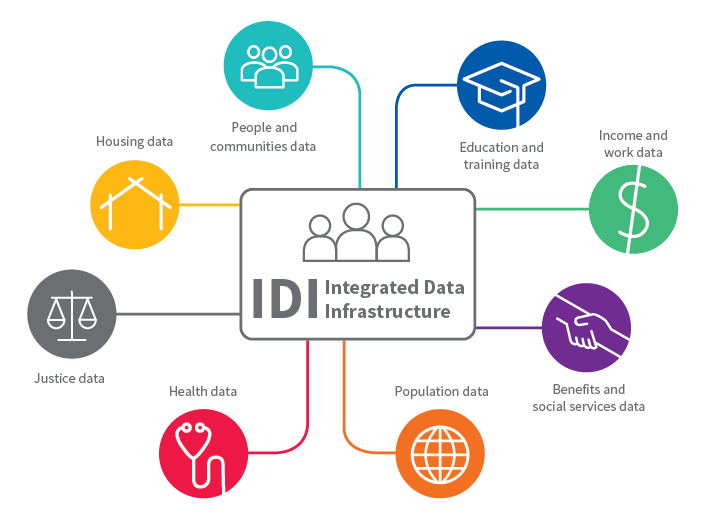
\includegraphics[width=0.5\linewidth]{idi.png}
    \end{center}

    \begin{itemize}
        \item Large research database, de-identified microdata
        \item Cross-sector research
    \end{itemize}
\end{frame}


\begin{frame}
    \frametitle{What's in the IDI?}

    \begin{itemize}
        \item $\approx{}50,000$ variables, $\approx{}1,000$ datasets
        \item Data dictionaries available in Data Lab
        \item ``Is information on X available in the IDI?''
        \item Can we build a searchable index?
    \end{itemize}
\end{frame}

\section{The data}

\begin{frame}
    \frametitle{IDI data sets}

    \begin{itemize}
        \item Admin datasets linkable at the individual level
        \item \emph{Clean} contains the routinely (3x yearly) updated data
        \item \emph{Adhoc} contains one-off or more frequently updated data (often with timestamped names)\\[2em]
        \item[$\Rightarrow$] Generate a list of variables from the schema
    \end{itemize}

\end{frame}

\begin{frame}
    \frametitle{Data dictionaries}

    \begin{itemize}
        \item Excel workbooks
        \begin{itemize}
            \item Detailed descriptions
            \item Variable names, coding information, etc.
        \end{itemize}
        \item Independent update/maintenance across agencies
        \begin{itemize}
            \item Inconsistent formats, structures, typos/errors, etc.
            \item Duplicated templates $\Rightarrow$ duplicated errors
        \end{itemize}
        \item Only available to approved, existing researchers
    \end{itemize}

\end{frame}


\begin{frame}
    \frametitle{Other data sources}

    \begin{itemize}
        \item Manually curated datasets by us
        \item Bridge the gap between IDI schema and data dictionaries\\[2em]
        \item Lists of collections without dictionaries
        \item Renamed datasets/variables
        \item Agency names and associated collections
        \item Regex patterns for date-stamped naming conventions
    \end{itemize}
\end{frame}

\begin{frame}
    \frametitle{Data hierarchy}

    \begin{center}

        \begin{align*}
            \overbracket[0.5pt]{\strut
            \text{Agency} \rightarrow
                \text{Collection}}^{\text{Manual}}
            \rightarrow
                    \underbracket[0.5pt]{\overbracket[0.5pt]{\strut
                    \text{Dataset} \rightarrow \text{Variable}
                    }^{\text{SQL Schema}}
                    }_{\text{Variables sheet}} \\[-1em]
                \hphantom{\text{Agency} \rightarrow}
                \underbracket[0.5pt]{
                \underbracket[0.5pt]{\hphantom{
                    \text{Collection} \rightarrow \text{Dataset}
                }}_{\text{Collections sheet / Manual}}
                \hphantom{\rightarrow \text{Variable}}
                }_{\text{Data dictionaries}}
        \end{align*}
    \end{center}
\end{frame}

\section{Tools}

\begin{frame}
    \frametitle{Data preparation}

    \begin{columns}
        \begin{column}{0.4\textwidth}
            \centering
            \includegraphics[width=0.7\linewidth]{rlogo.png}
        \end{column}
        \begin{column}{0.6\textwidth}
            \begin{itemize}
                \item free, open-source
                \item can read/write many formats
                \item powerful data manipulation tools
                \item easy to script
            \end{itemize}
        \end{column}
    \end{columns}
\end{frame}

\begin{frame}
    \frametitle{Deployment}

    \begin{columns}
        \begin{column}{0.4\textwidth}
            \centering
            
\includegraphics[width=0.8\linewidth]{mysql.png}
        \end{column}
        \begin{column}{0.6\textwidth}
            \begin{itemize}
                \item cloud hosted (planetscale)
                \item structured data
                \item text search
            \end{itemize}
        \end{column}
    \end{columns}

    \begin{columns}
        \begin{column}{0.4\textwidth}
            \centering
            
\includegraphics[width=0.7\linewidth]{nextjs.png}
        \end{column}
        \begin{column}{0.6\textwidth}
            \begin{itemize}
                \item Hosted on Vercel (free!)
                \item Easy to set-up and deploy
                \item Javascript framework (ReactJS)
            \end{itemize}
        \end{column}
    \end{columns}
\end{frame}

\section{The wrangling process}

\begin{frame}
    \frametitle{Read data dictionaries}

    \begin{itemize}
        \item \prog{R} script to parse Excel workbooks
        \item Extract collection, dataset, and variable metadata
        \item Detect issues/errors - modify script or fix manually
        \begin{itemize}
            \item After updating, sent back to Stats NZ
            \item More complex issues returned to Stats NZ to fix
        \end{itemize}
        \item Identify issues e.g., duplicate variables
    \end{itemize}
\end{frame}

\begin{frame}
    \frametitle{Read SQL variable list}

    \begin{itemize}
        \item All refreshes and adhoc lists
        \item Contains database, table, variable name
        \item Some info about variable type/size
    \end{itemize}
\end{frame}

\begin{frame}
    \frametitle{Combine with metadata}

    \begin{itemize}
        \item Link variables and datasets (some regex)
        \item Link datasets with collections (some manual)
        \item Link collections and agencies
        \item Store other metadata (e.g., name changes)
        \item Clean up duplicates, formatting, special characters
        \item Write to MySQL database
    \end{itemize}
\end{frame}

\section{Demo}


{ % all template changes are local to this group.
\setbeamertemplate{navigation symbols}{}
\begin{frame}<article:0>[plain]
    \begin{tikzpicture}[remember picture,overlay]
        \node[at=(current page.center)] {
            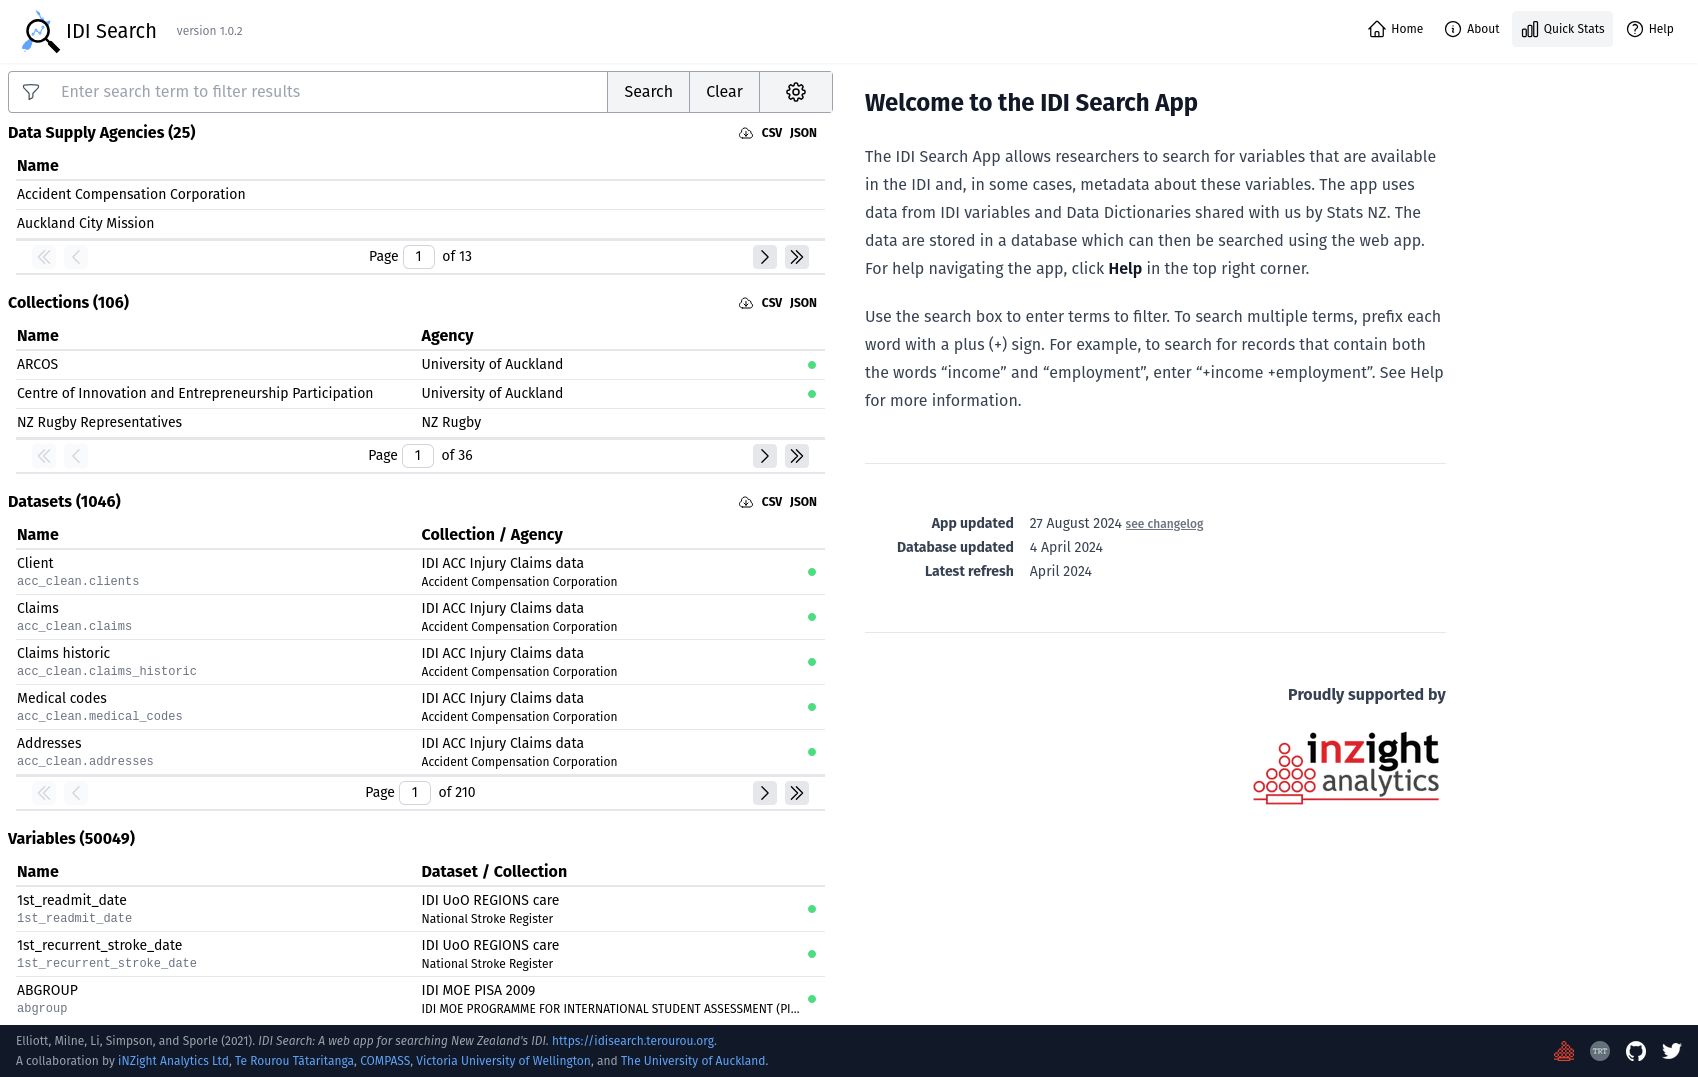
\includegraphics[keepaspectratio,
            width=\paperwidth,
            height=\paperheight]{demo1.png}
            };
    \end{tikzpicture}
\end{frame}


}

\section{Conclusion}

\begin{frame}
    \frametitle{Conclusion}

    
\includegraphics[width=\linewidth]{conc1.png}

    \begin{itemize}
        \item 10-30 users per day (~200 users per month)
        \item Listed as a go-to resource for new researchers
        \item Database funded by Stats NZ
        \item Data dictionary coverage increased, quality improved
        \item Mentioned in `Intro to the IDI' training
    \end{itemize}
\end{frame}

\begin{frame}
    \frametitle{Future Work}

    \begin{itemize}
        \item Automate data dictionary update/processing
        \item Secure funding for ongoing, routine updates
        \item New features
    \end{itemize}
\end{frame}

\setbeamertemplate{headline}{}
\setbeamertemplate{footline}{}
\begin{frame}

    \begin{center}
        
\includegraphics[width=3cm]{idisearch}\\
        \url{idisearch.terourou.org}\\
        \url{github.com/tmelliott/idi-search-app}
    \end{center}
\end{frame}

\end{document}
